\begin{blocksection}
\question Write a function, \lstinline$all_paths$ that takes in a tree, \lstinline$t$, and returns a list of paths from the root to each leaf.
For example, if we called \lstinline$all_paths(t)$ on the following tree:

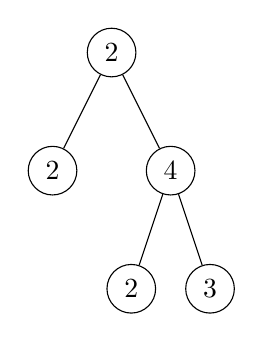
\begin{tikzpicture}[scale=1, transform shape]
\tikzstyle{level 2}=[sibling distance=10mm]
    \node [circle, draw] (z){$2$}
        child {node [circle, draw] (a) {$2$}}
        child {node [circle, draw] (d) {$4$}
            child {node [circle, draw] (g) {$2$}}
            child {node [circle, draw] (g) {$3$}}
        };
\end{tikzpicture}
\\\lstinline$all_paths(t)$ would return \lstinline$[[2, 2], [2, 4, 2], [2, 4, 3]].$
\newline

\begin{lstlisting}
def all_paths(t):
    paths = []
    if ________________________________________
        _______________________________________
    else:
        _______________________________________
            ___________________________________
                _______________________________
    return paths
\end{lstlisting}

\begin{solution}
\begin{lstlisting}
def all_paths(t):
    paths = []
    if is_leaf(t):
        paths.append([label(t)])
    else:
        for b in branches(t):
            for path in all_paths(b):
                paths.append([label(t)] + path)
    return paths
\end{lstlisting}

\textbf{Explanation:}
\newline
We begin by making a list to contain all the paths.
\newline
If the tree is a leaf, the root is a leaf, so the only path is \lstinline$[label(t)]$.
\newline
Otherwise, for each branch in the tree, we can use recursion to generate all the paths that extend from that branch to a leaf.
\newline
Finally, we combine the root label with each branch-starting path to make it a path from the root to a leaf.
\newline
Append every path like this to \lstinline$paths$, and we have created a list of all paths!
\end{solution}
\end{blocksection}

\begin{blocksection}
\begin{guide}
  \textbf{Teaching Tips}
  \begin{itemize}
      \item Variants of path problems commonly appear on exams! This problem covers the basic structure for all path problems, so make sure students understand and remember its format.
      \item In general, path problems involve two for loops, one iterating through branches and one iterating through a recursive call to a branch.
      \item A common mistake is for students to \lstinline$return [label(t)]$ instead of \lstinline$return [[label(t)]]$ for the base case. You can try writing the first option on "accident" to see if students will notice the error!
      \item The recursive leap of faith will help a lot for understanding path problems, particularly in the nested for loop.
      \begin{itemize}
        \item If students struggle to understand the solution, try writing out what \lstinline$all_paths(b)$ looks like by the leap of faith and show how why we append \lstinline$[label(t)]$ to each path in it before appending the path to paths.
      \end{itemize}
  \end{itemize}
\end{guide}
\end{blocksection}
